% !Mode:: "TeX:UTF-8"
% Translator: Yujun Li 
\chapter{\glsentrytext{representation_learning}}
\label{chap:representation_learning}
在本章中,首先我们会讨论学习表示是什么意思,以及表示的概念如何有助于深度框架的设计。
我们探讨学习算法如何在不同任务中共享统计信息,包括使用无监督任务中的信息进行监督任务。
共享表示有助于处理多模式或多领域,或是将已学到的知识转移到样本很少或没有,但任务表示存在的任务上。
最后,我们回溯去探讨\gls{representation_learning}成功的原因,从\gls{distributed_representation}\citep{Hinton-et-al-PDP1986}和深度表示的理论优势,到数据生成过程基本假设的更一般概念,特别是观测数据的基本成因。


很多信息处理任务,非常容易或者非常困难取决于信息是如何表示的。
这是一个普适于日常生活,普适于计算机科学的基本原则,也普适于机器学习。
例如,对于人而言,使用长除法计算210除以6非常直观。
但如果使用罗马数字表示,这个问题就没那么直观了。
大部分现代人在计算CCX除以VI时,都会将其转化成阿拉伯数字,从而使用位值系统的长除法。
更具体地,我们可以量化使用合适或不合适表示时,不同操作的渐近运行时间。
例如,插入一个数字到有序表中的正确位置,如果该数列表示为链表,那么所需时间是$O(n)$;如果该数列表示为红黑树,那么只需要$O(\log n)$的时间。

% -- 517 --

在机器学习中,如何判断一种表示比另一种表示更好呢?
一般而言,一个好的表示可以使随后的学习任务更容易。
选择什么表示通常取决于随后的学习任务。


我们可以将\gls{supervised_learning}训练的\gls{feedforward_network}视为一种\gls{representation_learning}。
具体地,网络的最后一层通常是\gls{linear_classifier},如\gls{softmax_chap15}回归分类器。
网络的其余部分学习出分类器输入的表示。
监督准则下的训练自然会使得每个\gls{hidden_layer}(比较接近顶层的\gls{hidden_layer})的表示趋向于具有使训练任务更容易的性质。
例如,输入特征线性不可分的类别可能在最后一个\gls{hidden_layer}变成线性可分的。
原则上,最后一层可以是另一种模型,如\gls{nearest_neighbor}分类\citep{SalakhutdinovR2007-small}。
倒数第二层的特征应该根据最后一层的类型学习不同的性质。


\gls{feedforward_network}的监督训练没有明确强加任何条件给学习的中间特征。
其他的\gls{representation_learning}算法往往会以某种特定的方式明确设计的表示。
例如,我们想要学习更容易估计密度的表示。
具有更多独立元素的分布会更容易建模,因此,我们可以设计鼓励表示向量$\Vh$中元素独立的目标函数。
就像监督网络,无监督深度学习算法有一个主要的训练目标,但也额外地学习出了表示。
不论该表示是如何得到的,它都可以运用于其他任务。
另外,很多任务(有些是\gls{supervised}的,有些是\gls{unsupervised}的)可以通过共享的内部表示一起学习。


大多数\gls{representation_learning}算法都会权衡,保留尽可能多和输入相关的信息,还是追求良好的性质(如独立性)。


\gls{representation_learning}特别有趣,因为它提供了一种方法来进行\gls{unsupervised_learning}和\gls{semi_supervised_learning}。
我们通常会有非常大量的未标记的训练数据和相对较少的有标记的训练数据。
在非常有限的标记数据集上\gls{supervised_learning}通常会导致过拟合。
\gls{semi_supervised_learning}通过进一步学习未标记的数据,来解决过拟合的问题。
具体地,我们可以从未标记的数据上学习出很好的表示,然后用这些表示来解决\gls{supervised_learning}问题。


人类和动物能够从非常少的标记样本中学习。
我们至今仍不知道这是如何做到的。
有许多假说解释人类的卓越学习能力——例如,大脑可能使用了大量的分类器或者贝叶斯推断技术。
一种流行的假说是,大脑能够利用\gls{unsupervised_learning}和\gls{semi_supervised_learning},使用很多方法来利用无标记的数据。
在本章中,我们主要探讨未标记的数据可以学习出更好的表示。

% -- 518 --

\section{贪心地逐层\glsentrytext{unsupervised_pretraining} }
\label{sec:greedy_layer_wise_unsupervised_pretraining}
\gls{unsupervised_learning}在\gls{DNN}的复兴历史上起到了关键作用,使研究者首次可以训练不含诸如\gls{convolution}或者\gls{recurrence}这类特殊结构的深度监督网络。
我们将这一过程称为\firstgls{unsupervised_pretraining},或者更精确地,\firstgls{greedy_layer_wise_unsupervised_pretraining}。
此过程时一个任务(\gls{unsupervised_learning},尝试抓住输入分布的形状)的表示如何有助于另一个任务(具有相同输入域的\gls{supervised_learning})的典型示例。


\gls{greedy_layer_wise_unsupervised_pretraining}依赖于单层\gls{representation_learning}算法,例如\glssymbol{RBM},单层\gls{AE},\gls{sparse_coding}模型,或其他学习隐表示的模型。
每一层使用\gls{unsupervised_learning}\gls{pretraining},输入前一层的输出,输出数据的新型表示,新型表示的分布(或者是和其他变量,如要预测的类别,的关系)有可能是很简单的。
如\algref{alg:pretraining}所示正式的表述。

\begin{algorithm}
\caption{ {\em \gls{greedy_layer_wise_unsupervised_pretraining}的协定}\\
给定如下:无监督特征学习算法$\CalL$,$\CalL$使用训练集样本并返回\gls{encoder}或特征函数$f$。
原始输入数据是$\MX$,每行一个样本,并且$f^{(1)}(\MX)$是第一阶段\gls{encoder}关于$\MX$的输出。
在执行\gls{fine_tune}的情况下,我们使用学习者$\CalT$,并使用初始函数$f$,输入样本$\MX$(以及在监督\gls{fine_tune}情况下关联的目标$\MY$),并返回细调好函数。 阶段数为$m$。
}
\label{alg:pretraining}
\begin{algorithmic}
\STATE $f \leftarrow$ 恒等函数
\STATE $\tilde{\MX} = \MX$
\FOR {$k=1, \ldots, m$}
  \STATE $f^{(k)} = {\CalL}(\tilde{\MX})$
  \STATE $f \leftarrow f^{(k)} \circ f$
  \STATE $\tilde{\MX} \leftarrow f^{(k)}(\tilde{\MX})$
\ENDFOR
\IF {\em fine-tuning}
  \STATE $f \leftarrow {\CalT}(f,\MX,\MY)$
\ENDIF
\STATE {\bf Return} $f$
\end{algorithmic}
\end{algorithm}


基于无监督标准的贪心逐层训练过程,早已被用来规避监督问题中深度网络难以联合训练多层的问题。
这种方法至少可以追溯神经认知机\citep{Fukushima75}。
深度学习的复兴始于2006年发现,这种贪心学习的过程能够为多层联合训练过程找到一个好的初始值,甚至可以成功训练全连接的结构\citep{Hinton06-small,Hinton-Science2006,HintonG2006,Bengio-nips-2006,ranzato-07-small}。
在此发现之前,只有深度卷积网络或深度循环网络这类特殊结构的深度网络被认为是有可能训练的。
现在我们知道训练全连接的深度结构,\gls{greedy_layer_wise_unsupervised_pretraining}不是唯一的方法,但无监督提前训练是第一个成功的方法。


\gls{greedy_layer_wise_unsupervised_pretraining}被称为\firstgls{greedy}的,是因为它是一个\firstgls{greedy_algorithm},
这意味着它每次独立地优化一个解决方案,而不是联合优化所有的解决方案。
它被称为\firstgls{layer_wise},是因为这些独立的解决方案是网络层。
具体地,\gls{greedy_layer_wise_unsupervised_pretraining}每次处理一层网络,训练第$k$层时保持前面的网络层不变。
特别地,低层网络(最先训练的)不会在引入高层网络后进行调整。
它被称为\firstgls{unsupervised}的,是因为每一层用\gls{unsupervised}\gls{representation_learning}算法训练。
然而,它也被称为\firstgls{pretraining},是因为它只是在联合训练算法\textbf{\gls{fine_tune}}所有层之前的第一步。
在\gls{supervised_learning}任务中,它可以被看作是正则项(在一些实验中,\gls{pretraining}不能降低训练误差,但能降低测试误差)和参数初始化的一种形式。

% -- 519 --

通常而言,``\gls{pretraining}''不仅单指\gls{pretraining}阶段,也指结合\gls{pretraining}和\gls{supervised_learning}的整个两阶段学习过程。
\gls{supervised_learning}阶段可能会使用\gls{pretraining}阶段得到的顶层特征训练一个简单分类器,或者可能会监督\gls{fine_tune}\gls{pretraining}阶段得到的整个网络。
不管采用什么类型的\gls{supervised_learning}算法和模型,在大多数情况下,整个训练过程几乎是相同的。
虽然\gls{unsupervised_learning}算法的选择将明显影响到细节,但是大多数\gls{unsupervised}\gls{pretraining}应用都遵循这一基本方法。


\gls{greedy_layer_wise_unsupervised_pretraining}也能用作其他\gls{unsupervised_learning}算法的初始化,比如深度\gls{AE}\citep{Hinton-Science2006}和具有很多\gls{latent_variable}层的概率模型。
这些\gls{model}包括\gls{DBN}\citep{Hinton06-small}和\gls{DBM}\citep{Salakhutdinov+Hinton-2009-small}。
这些\gls{DGM}会在\chapref{chap:deep_generative_models}讨论。


正如\secref{sec:supervised_pretraining}所探讨的,也可以进行贪心逐层\emph{监督}\gls{pretraining}。
这建立在训练浅层模型比\gls{deep_model}更容易的前提下,而该前提似乎在一些情况下已被证实\citep{Erhan+al-2010-small}。


\subsection{何时以及为何\glsentrytext{unsupervised_pretraining}有效?}
\label{sec:when_and_why_does_unsupervised_pretraining_work}
在很多分类任务中,\gls{greedy_layer_wise_unsupervised_pretraining}能够在\gls{test_error}上获得重大提升。
这一观察结果始于2006年对\gls{DNN}的重新关注\citep{Hinton06-small,Bengio-nips-2006,ranzato-07-small}。
然而,在很多其他问题上,\gls{unsupervised_learning}不能带来改善,甚至还会带来明显的负面影响。
\cite{Ma-et-al-2015}研究了\gls{pretraining}对\gls{ML_model}在化学活性预测上的影响。
结果发现,平均而言\gls{pretraining}是有轻微负面影响的,但在有些问题上会有显著帮助。
由于\gls{unsupervised_pretraining}有时有效,但经常也会带来负面效果,因此很有必要了解它何时有效以及有效的原因,以确定它是否适合用于特定的任务。

% -- 520 --

首先,要注意的是这个讨论大部分都是针对\gls{greedy_unsupervised_pretraining}而言。
还有很多其他完全不同的方法用于训练\gls{semi_supervised_learning}\gls{NN},比如\secref{sec:adversarial_training}介绍的\gls{virtual_adversarial_training}。
我们还可以在训练\gls{supervised_model}的同时训练\gls{AE}或\gls{generative_model}。
这种单阶段方法的例子包括\gls{discriminative_RBM}\citep{Larochelle+Bengio-2008}和梯形网络\citep{Rasmus-et-al-arxiv2015},整体目标是两项之和(一个使用标签,另一个使用输入)。


\gls{unsupervised_pretraining}结合了两种不同的想法。
第一,它利用了\gls{DNN}对初始参数的选择,可以对模型有着显著的\gls{regularization}效果(在较小程度上,可以改进优化)的想法。
第二,它利用了更一般的想法,学习\gls{input_distribution}有助于学习从\gls{input}到\gls{output}的映射。

% -- 521 --

这两个想法都涉及到多个未能完全理解的机器学习算法之间的相互作用。


第一个想法,\gls{DNN}初始参数的选择对其性能具有很强的\gls{regularization}效果,是最不容易理解的。
在\gls{pretraining}变得流行时,在一个位置初始化模型被认为会使其接近某一个\gls{local_minimum},而不是另一个\gls{local_minimum}。
如今,\gls{local_minima}不再被认为是\gls{NN}优化中的严重问题。
现在我们知道标准的\gls{NN}训练过程通常不会到达任何类型的极值点。
仍然可能的是,\gls{pretraining}会初始化模型到一个可能不会探索的位置——例如,某种区域,其中\gls{cost_function}从一个样本点到另一个样本点变化很大,\gls{minibatch}只能提供\gls{noise}严重的梯度估计,或是某种区域中的\gls{hessian}矩阵条件数是病态的,梯度下降法必须使用非常小的步长。
然而,我们很难准确判断\gls{supervised_learning}期间\gls{pretraining}参数的哪些部分应该保留。
这是现代方法通常同时使用\gls{unsupervised_learning}和\gls{supervised_learning},而不是依序使用两个学习阶段的原因之一。
除去让\gls{supervised_learning}阶段保持\gls{unsupervised_learning}阶段所提取信息的复杂方法,我们还可以简单地固定特征提取器的参数,仅仅将\gls{supervised_learning}作为顶层特征的分类器。

另一个想法,学习算法可以使用\gls{unsupervised}阶段学习的信息,更好地执行\gls{supervised_learning}阶段,已经被很好地理解了。
基本想法是对于\gls{unsupervised}任务有用的一些特征对于\gls{supervised_learning}任务也可能是有用的。
例如,如果我们训练汽车和摩托车图像的生成模型,它需要知道轮子的概念,以及一张图中应该有多少个轮子。
如果我们幸运,已经知道轮子采取一种易于被\gls{supervised_learning}获取的表示形式,那么这个任务会变得容易。
然而还未能从理论层面上证明,因此并不总是能够预测哪种任务能以这种形式从\gls{unsupervised_learning}中受益。
这种方法高度依赖于具体使用的模型。
例如,如果我们希望为\gls{pretraining}的特征添加\gls{linear_classifier},那么学习到的特征必须使底层类别线性可分。
这些性质通常自然地发生,但并非总是这样。
这是另一个\gls{supervised}和\gls{unsupervised_learning}同时训练更可取的原因——输出层施加的约束很自然地从一开始就包括在内。

% -- 522 --

从\gls{unsupervised_pretraining}作为学习表示的角度来看,我们可以期望\gls{unsupervised_pretraining}在初始表示较差的情况下更有效。
一个重要的例子是\gls{word_embeddings}。
使用\gls{one_hot}向量表示的词不是具有很多信息,因为任意两个不同的\gls{one_hot}向量之间的距离(平方$L^2$距离都是$2$ )都是相同的。
学习到的\gls{word_embeddings}自然会用它们彼此之间的距离来编码词之间的相似性。
因此,\gls{unsupervised_pretraining}在处理单词时特别有用。
然而在处理图像时是不太有用的,可能是因为图像已经在一个很丰富的向量空间中,其中的距离只能提供低质量的相似性度量。


从\gls{unsupervised_pretraining}作为正则项的角度来看,我们可以期望\gls{unsupervised_pretraining}在标记样本数量非常小时很有帮助。
因为\gls{unsupervised_pretraining}添加的信息来源于未标记的数据,所以当未标记样本的数量非常大时,我们也可以期望\gls{unsupervised_pretraining}的效果最好。
\gls{unsupervised_pretraining}的大量未标记样本和少量标记样本构成的\gls{semi_supervised_learning}的优势在2011年特别明显。
\gls{unsupervised_pretraining}赢得了两个国际\gls{transfer_learning}比赛\citep{UTLC+LISA-2011-small,goodfellow+all-NIPS2011},在该设定中,目标任务中标记样本的数目很少(每类几个到几十个)。
这些效果也出现在被\citep{paine2014analysis}仔细控制的实验中。


还有一些其他的因素可能会涉及。
例如,当要学习的函数非常复杂时,\gls{unsupervised_pretraining}可能会非常有用。
\gls{unsupervised_learning}不同于\gls{weight_decay}这样的\gls{regularizer},它不偏向于学习一个简单的函数,而是学习对\gls{unsupervised_learning}任务有用的特征函数。
如果真实的底层函数是复杂的,并且由\gls{input_distribution}的规律塑造,那么\gls{unsupervised_learning}更适合作为\gls{regularizer}。


除了这些注意事项外,我们现在分析一些\gls{unsupervised_pretraining}改善性能的成功示例,并解释这种改进发生的已知原因。
\gls{unsupervised_pretraining}通常用来改进分类器,并且从减少测试误差的观点来看是很有意思的。
然而,\gls{unsupervised_pretraining}还有助于分类以外的任务,并且可以用于改进优化,而不仅仅只是作为正规化项。
例如,它可以提高\gls{DAE}的训练和测试\gls{reconstruction_error}\citep{Hinton-Science2006}。

% -- 523 --

\cite{Erhan+al-2010-small}进行了许多实验来解释\gls{unsupervised_pretraining}的几个成功点。
对训练误差和测试误差的改进都可以解释为,\gls{unsupervised_pretraining}将参数引入到了可能不会探索的区域。
\gls{NN}训练是非确定性的,并且每次运行都会收敛到不同的函数。
训练可以停止在梯度变小的点;也可以\gls{early_stopping}结束训练,以防过拟合;还可以停止在梯度很大,但由于诸如随机性或\gls{hessian}矩阵\gls{poor_conditioning}等问题难以找到合适下降方向的点。
经过\gls{unsupervised_pretraining}的神经网络会一致地停止在一片相同的区域,但未经过\gls{pretraining}的\gls{NN}会一致地停在另一个区域。
参看\figref{fig:chap15_isomap}了解这种现象。
经过\gls{pretraining}的网络到达的区域是较小的,这表明\gls{pretraining}减少了估计过程的方差,这进而又可以降低严重过拟合的风险。
换言之,\gls{unsupervised_pretraining}将\gls{NN}参数初始化到它们不易逃逸的区域,并且遵循这种初始化的结果更加一致,和没有这种初始化相比,结果很差的可能性更低。


\cite{Erhan+al-2010-small}也回答了\emph{何时}\gls{pretraining}效果最好——预训练的网络越深,\gls{test_error}的均值和方差下降得越多。
值得注意的是,这些实验是在训练非常深层网络的现代方法发明和流行(\gls{ReLU},\gls{dropout}和\gls{batch_normalization})之前进行的,因此对于\gls{unsupervised_pretraining}与当前方法的结合,我们所知甚少。


一个重要的问题是\gls{unsupervised_pretraining}是如何作为\gls{regularizer}的。
一个假设是,\gls{pretraining}鼓励学习算法发现与生成观察数据的根本原因相关的特征。
这是激励除\gls{unsupervised_pretraining}之外的许多其它算法的重要思想,将会在\secref{sec:semi_supervised_disentangling_of_causal_factors}中进一步讨论。


与\gls{unsupervised_learning}的其它形式相比,\gls{unsupervised_pretraining}的缺点是其使用了两个单独的训练阶段。
很多\gls{regularization}技术都具有一个优点,允许用户调整单一\gls{hyperparameter}控制\gls{regularization}的强度。
\gls{unsupervised_pretraining}没有一种明确的方法,调整\gls{unsupervised}阶段\gls{regularization}的强度。
相反,\gls{unsupervised_pretraining}有许多超参数,但其效果只能之后度量,通常难以提前预测。
当我们同时执行\gls{unsupervised}和\gls{supervised_learning}而不使用\gls{pretraining}策略时,会有单个超参数(通常是附加到无监督损失的系数)控制无监督目标正则化监督模型的强度。
减少该系数,总是能够可预测地获得较少\gls{regularization}强度。
在\gls{unsupervised_pretraining}的情况下,没有一种灵活适应\gls{regularization}强度的方式——要么监督模型初始化为\gls{pretraining}的参数,要么不是。

% -- 524 --

\begin{figure}[!htb]
\ifOpenSource
\centerline{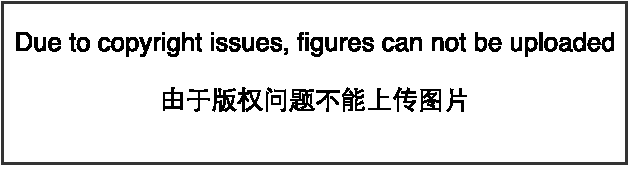
\includegraphics{figure.pdf}}
\else
\centerline{\includegraphics{Chapter15/figures/isomap_color}}
\fi
\caption{TODO}
\label{fig:chap15_isomap}
\end{figure}


具有两个单独的训练阶段的另一个缺点是每个阶段都具有自己的超参数。
第二阶段的性能通常不能在第一阶段期间预测,因此在第一阶段提出超参数和第二阶段根据反馈来更新之间存在较长的延迟。
最主要的方法是使用监督阶段验证集的误差来挑选\gls{pretraining}阶段的超参数,如\cite{Larochelle-jmlr-2009}中讨论的。
在实际中,有些超参数,如\gls{pretraining}迭代的次数,很方便在\gls{pretraining}阶段设定,在\gls{unsupervised}目标上使用提前停止。这个方法并不理想,但是计算上比使用监督目标代价小得多。

% -- 525 --

如今,大部分算法已经不使用\gls{unsupervised_pretraining}了,除了在自然语言处理领域,其中单词作为\gls{one_hot}向量的自然表示不能传达相似性信息,并且有非常多的未标记集可用。
在这种情况下,\gls{pretraining}的优点是可以对一个巨大的未标记集合(例如用包含数十亿单词的语料库)进行\gls{pretraining},学习良好的表示(通常是单词,但也可以是句子),然后使用该表示或\gls{fine_tune}表示,用于训练集样本很少的监督任务。
这种方法由\cite{CollobertR2008-small},\cite{Turian+Ratinov+Bengio-2010-small}和\cite{collobert2011natural}开创,至今仍在使用。


基于\gls{supervised_learning}的\gls{DL}技术,通过\gls{dropout}或\gls{batch_normalization}来\gls{regularization},能够在很多任务上达到人类级别的性能,但必须使用极大的标记数据集。
在中等大小的数据集(例如CIFAR-10和MNIST,每个类大约有5,000个标记的样本)上,这些技术的效果比\gls{unsupervised_pretraining}更好。
在极小的数据集,例如\gls{alternative_splicing_dataset},贝叶斯方法要优于基于\gls{unsupervised_pretraining}的方法\citep{Srivastava-master-small}。
由于这些原因,\gls{unsupervised_pretraining}已经不如以前流行。
然而,\gls{unsupervised_pretraining}仍然是深度学习研究历史上的一个重要里程碑,并继续影响当代方法。
\gls{pretraining}的想法已经推广到\secref{sec:supervised_pretraining}中讨论的\firstgls{supervised_pretraining},这是\gls{transfer_learning}中非常常用的方法。
\gls{transfer_learning}中的\gls{supervised_pretraining}流行\citep{Oquab-et-al-CVPR2014,yosinski-nips2014}于在ImageNet数据集上使用\gls{convolutional_network}\gls{pretraining}。
由于这个原因,实践者们公布了这些网络训练出的参数,就像自然语言任务公布\gls{pretraining}的单词向量一样\citep{collobert2011natural,Mikolov-et-al-ICLR2013}。

% -- 526 --

\section{\glsentrytext{transfer_learning}和\glsentrytext{domain_adaption}}
\label{sec:transfer_learning_and_domain_adaptation}
\gls{transfer_learning}和\gls{domain_adaption}指的是利用一个设定(分布$P_1$)中已经学到的内容去改善另一个设定(比如分布$P_2$)中的泛化情况。
这点概括了上一节提出的想法,在\gls{unsupervised_learning}和\gls{supervised_learning}之间转移表示。


在\firstgls{transfer_learning}中,\gls{learner}必须执行两个或更多个不同的任务,但是我们假设能够解释$P_1$变化的许多因素和学习$P_2$需要抓住的变化相关。
这通常能够在\gls{supervised_learning}的情况中理解,输入是相同的,但是输出具有不同的性质。
例如,我们可能在第一种设定中学习了一组视觉类别,比如猫和狗,然后在第二种设定中学习一组不同的视觉类别。
如果第一种设定(从$P_1$采样)中具有非常多的数据,那么这有助于在$P_2$抽取到的非常少的样本中快速泛化。
许多视觉类别\emph{共享}一些低级概念,比如边缘,视觉形状,几何变化,照明变化的影响等。
一般而言,当存在对不同设定或任务有用,且对应多个设定的潜在因素的特征时,\gls{transfer_learning},\gls{multitask_learning}(\secref{sec:multitask_learning})和\gls{domain_adaption}可以使用\gls{representation_learning}来实现。
如\figref{fig:chap7_multi_factor_output}所示,具有共享底层和任务相关上层的学习框架。


然而,有时不同任务之间共享的不是输入的语义,而是输出的语义。
例如,语音识别系统需要在输出层产生有效的句子,但是输入附近的较低层可能需要识别相同音素或子音素发音的非常不同的版本(这取决于哪个人正在说话)。
在这样的情况下,共享神经网络的上层(输出附近)和进行任务特定的预处理是有意义的,如\figref{fig:chap15_multi_task_input}所示。

\begin{figure}[!htb]
\ifOpenSource
\centerline{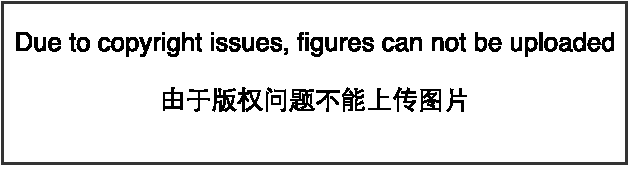
\includegraphics{figure.pdf}}
\else
\centerline{\includegraphics{Chapter15/figures/multi_task_input}}
\fi
\caption{TODO}
\label{fig:chap15_multi_task_input}
\end{figure}

在\firstgls{domain_adaption}的相关情况下,任务(和最优的输入输出映射)在每个设定之间保持相同,但是\gls{input_distribution}稍有不同。 
例如,考虑情感分析的任务,包括判断评论是否表达积极或消极情绪。 
网上的评论来自许多类别。
在书,视频和音乐等媒体内容上训练的顾客评论情感预测器,被用于分析诸如电视机或智能电话的消费电子产品的评论时,\gls{domain_adaption}情景可能会出现。
可以想象,存在一个潜在的函数可以判断任何语句是正面的,中性的还是负面的,但是词汇和风格可能会因领域而有差异,使得跨域的泛化训练变得更加困难。
简单的\gls{unsupervised_pretraining}(\gls{DAE})已经能够非常成功地用于\gls{domain_adaption}的情感分析\citep{Glorot+al-ICML-2011}。

% -- 527 --

一个相关的问题是\firstgls{concept_drift},我们可以将其视为一种\gls{transfer_learning},因为数据分布随时间而逐渐变化。
\gls{concept_drift}和\gls{transfer_learning}都可以被视为\gls{multitask_learning}的特定形式。
短语``\gls{multitask_learning}''通常指\gls{supervised_learning}任务,而\gls{transfer_learning}中更一般的概念也适用于\gls{unsupervised_learning}和\gls{RL}。

在所有这些情况下,目标是利用第一个设定下的数据优势,提取在第二种设定中学习时或直接进行预测时可能有用的信息。
\gls{representation_learning}的核心思想是相同的表示可能在两种设定中都是有用的。
两个设定使用相同的表示,使得表示可以受益于两个任务的训练数据。


如前所述,\gls{unsupervised}\gls{DL}用于\gls{transfer_learning}已经在一些机器学习比赛中取得了成功\citep{UTLC+LISA-2011-small,goodfellow+all-NIPS2011}。
这些比赛中的某一个实验设定如下。
首先每个参与者获得一个第一种设定(来自分布$P_1$)的数据集,其中含有一些类别的样本。
参与者必须用这个来学习一个良好的特征空间(将原始输入映射到某种表示),这样当我们将这个学习到的变换用于来自迁移设定(分布$P_2$)的输入时,\gls{linear_classifier}可以在有标记样本很少的训练集上训练,泛化。
这个比赛中最引人注目的结果之一是,学习表示的网络架构越深(在第一个设定$P_1$中的数据使用纯无监督的方式学习),在第二个设定(迁移)$P_2$的新类别上学习到的曲线就越好。
对于深度表示而言,迁移任务只需要较少的标记样本就能明显地渐近泛化性能。

% -- 528 --

\gls{transfer_learning}的两种极端形式是\firstgls{one_shot_learning}和\firstgls{zero_shot_learning},有时也被称为\firstgls{zero_data_learning}。
只有一个标记样本的迁移任务被称为\gls{one_shot_learning};没有标记样本的迁移任务被称为\gls{zero_shot_learning}。


因为第一阶段学习出的表示就可以清楚地分离类别,所以\gls{one_shot_learning}\citep{Fei-Fei+al-2006}是可能的。
在\gls{transfer_learning}阶段,仅需要一个标记样本来推断表示空间中聚集在相同点周围的许多可能的测试样本的标签。
这使得在学习到的表示空间中,对应于不变性的变化因子已经与其它因子完全分离,在区分某些类别的对象时,我们以哪种方式学习到哪些因素具有决定意义。


考虑一个\gls{zero_shot_learning}设定的例子,\gls{learner}已经读取了大量文本,然后要解决对象识别的问题。
如果文本足够好地描述了对象,那么即使没有看到某对象的图像,也能识别该对象。
例如,已知猫有四条腿和尖尖的耳朵,那么\gls{learner}可以在没有见过猫的情况下猜测该图像是猫。


只有在训练时使用了额外信息,\gls{zero_data_learning}\citep{Larochelle2008}和\gls{zero_shot_learning}\citep{Palatucci2009,Socher-2013}才是有可能的。
我们可以认为\gls{zero_data_learning}场景包含三个随机变量:传统输入$\Vx$,传统输出或目标$\Vy$,以及描述任务的附加随机变量,$T$。
该模型被训练来估计条件分布$p(\Vy \mid \Vx, T)$,其中$T$是我们希望执行的任务的描述。
在我们的例子中,读取猫的文本信息然后识别猫,输出是二元变量$y$,$y=1$表示``是'',$y=0$表示``不是''。
任务变量$T$表示要回答的问题,例如``这个图像中是否有猫?''
如果训练集包含和$T$在相同空间的\gls{unsupervised}对象样本,我们也许能够推断未知的$T$实例的含义。
在我们的例子中,没有提前看到猫的图像而去识别猫,拥有一些未标记的文本数据包含句子诸如``猫有四条腿''或``猫有尖耳朵'',对于学习非常有帮助。

% -- 529 --

\gls{zero_shot_learning}要求$T$被表示为某种泛化的形式。
例如,$T$不能仅是指示对象类别的\gls{one_hot}。
通过使用每个类别词的\gls{word_embeddings}表示,\cite{Socher-2013}提出了对象类别的\gls{distributed_representation}。


一种类似的现象出现在\gls{machine_translation}中\citep{Klementiev-et-al-COLING2012,Mikolov-et-al-arxiv2013,Gouws-et-al-arxiv2014}:我们已经知道一种语言中的单词,和非语言语料库中学到的词与词之间的关系;另一方面,我们已经翻译了一种语言中的单词与另一种语言中的单词相关的句子。
即使我们可能没有将语言$X$中的单词$A$翻译成语言$Y$中的单词$B$的标记样本,我们也可以泛化并猜出单词$A$的翻译,这是由于我们已经学习了语言$X$和$Y$的\gls{distributed_representation},并且通过两种语言相匹配句子组成的训练样本,产生了关联于两个空间的连接(可能是双向的)。
如果联合学习三种所有成分(两种表示形式和它们之间的关系),那么这种迁移将会非常成功。


\gls{zero_shot_learning}是\gls{transfer_learning}的一种特殊形式。
同样的原理可以解释如何能执行\firstgls{multimodal_learning},学习两种模态的表示,和一种模态中的观察结果$\Vx$与另一种模态中的观察结果$\Vy$组成的对$(\Vx, \Vy)$之间的关系(通常是一个联合分布)\citep{Srivastava+Salakhutdinov-NIPS2012-small}。
通过学习所有的三组参数(从$\Vx$到它的表示,从$\Vy$到它的表示,以及两个表示之间的关系),一个表示中的概念被锚定在另一个表示中,反之亦然,从而可以有效地推广到新的对组。
这个过程如\figref{fig:chap15_maps_between_representations}所示。

\begin{figure}[!htb]
\ifOpenSource
\centerline{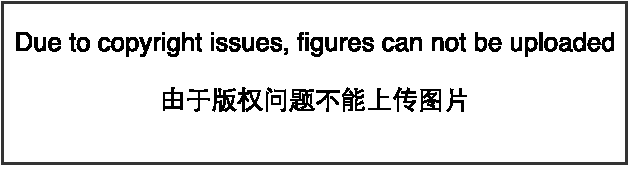
\includegraphics{figure.pdf}}
\else
\centerline{\includegraphics{Chapter15/figures/maps_between_representations}}
\fi
\caption{TODO}
\label{fig:chap15_maps_between_representations}
\end{figure}

% -- 530 --

\section{\glsentrytext{semi_supervised}解释因果关系}
\label{sec:semi_supervised_disentangling_of_causal_factors}
\gls{representation_learning}的一个重要问题是``什么原因能够使一个表示比另一个表示更好?''
一种假设是,理想表示中的特征对应到观测数据的根本成因,特征空间中不同的特征或方向对应着不同的原因,从而表示能够区分这些原因。
这个假设激励我们去寻找表示$p(\Vx)$的更好方法。
如果$\Vy$是$\Vx$的重要成因之一,那么这种表示也可能是计算$p(\Vy \mid \Vx)$的一种良好表示。
至少从20世纪90年代以来,这个想法已经指导了大量的\gls{DL}研究工作\citep{Becker92,hinton1999unsupervised}。
关于\gls{semi_supervised_learning}可以超过纯\gls{supervised_learning}的其他论点,请读者参考\cite{Chapelle-2006}的\secref{sec:historical_trends_in_deep_learning}。


在\gls{representation_learning}的其他方法中,我们大多关注易于建模的表示——例如,数据稀疏或是各项独立的情况。
能够清楚地分离出潜在因素的表示可能并不易于建模。
然而,该假设的激励\gls{semi_supervised_learning}使用无监督\gls{representation_learning}的一个更深层原因是,对于很多人工智能任务而言,有两个相随的特点:一旦我们能够获得观察结果基本成因的解释,那么将会很容易分离出个体属性。
具体来说,如果表示向量$\Vh$表示观察值$\Vx$的很多根本因素,输出向量$\Vy$是最为重要的原因之一,那么从$\Vh$预测$\Vy$会很容易。


首先,让我们看看$p(\RVx)$的\gls{unsupervised_learning}无助于学习$p(\RVy\mid\RVx)$时,\gls{semi_supervised_learning}为何失败。
考虑一种情况,$p(\RVx)$是均匀分布的,我们希望学习$f(\Vx) = \SetE[\RVy \mid \Vx]$。
显然,仅仅观察训练集的值$\Vx$不能给我们关于$p(\RVy \mid \RVx)$的任何信息。


接下来,让我们看看\gls{semi_supervised_learning}成功的一个简单例子。
考虑这样的情况,$\RVx$来自一个混合分布,每个$\RVy$值具有一个混合分量,如\figref{fig:chap15_mixture_model}所示。
如果混合分量很好地分出来了,那么建模$p(\RVx)$可以精确地指出每个分量的方向,每个类一个标记样本的训练集足以精确学习$p(\RVy \mid \RVx)$。
但是更一般地,什么能将$p(\RVy \mid \RVx)$和$p(\RVx)$关联在一起呢?

\begin{figure}[!htb]
\ifOpenSource
\centerline{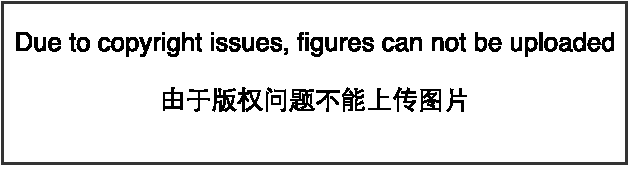
\includegraphics{figure.pdf}}
\else
\centerline{\includegraphics{Chapter15/figures/mixture_model_color}}
\fi
\caption{TODO}
\label{fig:chap15_mixture_model}
\end{figure}

如果$\RVy$与$\RVx$的成因之一非常相关,那么$p(\RVx)$和$p(\RVy \mid \RVx)$也会紧密关联,试图找到变化根本因素的无监督\gls{representation_learning}可能会有助于\gls{semi_supervised_learning}。

% -- 532 --

假设$\RVy$是$\RVx$的成因之一,让$\RVh$代表所有这些成因。
真实的生成过程可以被认为是根据这个\gls{directed_graphical_model}结构化出来的,其中$\RVh$是$\RVx$的因素:
\begin{equation}
	p(\RVh, \RVx) = p(\RVx \mid \RVh) p(\RVh).
\end{equation}
因此,数据的边缘概率是
\begin{equation}
	p(\Vx) = \SetE_{\RVh} p(\Vx \mid \Vh),
\end{equation}
从这个直观的观察,我们得出结论,$\RVx$最好可能的模型(从广义的观点)是会表示上述``真实''结构的,其中$\Vh$作为\gls{latent_variable}解释$\Vx$代表的观察变动。
上文讨论的``理想''的\gls{representation_learning}应该能够反映出这些隐变量。
如果$\RVy$是其中之一(或是紧密关联于其中之一),那么将很容易从这种表示中预测$\RVy$。
我们会看到给定$\RVx$下$\RVy$的条件分布通过\gls{bayes_rule}关联到上式中的分量:
\begin{equation}
	p(\RVy \mid \RVx) = \frac{ p(\RVx \mid \RVy) p(\RVy) }{p(\RVx)}.
\end{equation}
因此边缘概率$p(\RVx)$和条件概率$p(\RVy \mid \RVx)$密切相关,前者的结构信息应该有助于学习后者。
因此,在这些假设情况下,\gls{semi_supervised_learning}应该能提高性能。


一个重要的研究问题是,大多数观察是由极其大量的潜在成因形成的。
假设$\RVy = \RSh_i$,但是\gls{unsupervised_learning}并不知道哪一个是$\RSh_i$。
暴力求解\gls{unsupervised_learning}是学习一种表示,捕获\emph{所有}合理的重要生成因子$\RSh_j$,并将它们彼此区分开来,因此不管$\RSh_i$是否关联于$\RVy$,从$\RVh$预测$\RVy$都是容易的。

% -- 533 --

在实践中,暴力求解是不可行的,因为不可能捕获影响观察的所有或大多数变化。
例如,在视觉场景中,表示是否应该对背景中的所有最小对象进行编码?
一个有据可查的心理学现象是,人们不会察觉到环境中和他们所在进行的任务并不紧紧相关的变化——具体例子可参考\cite{simons1998failure}。
\gls{semi_supervised_learning}的一个重要研究前沿是确定每种情况下要编码的对象。
目前,处理大量潜在原因的两个主要策略是,同时使用\gls{unsupervised_learning}和\gls{supervised_learning},使模型捕获最相关的变动因素,或是使用纯\gls{unsupervised_learning}学习更大规模的表示。


\gls{unsupervised_learning}的一个新兴策略是修改确定哪些潜在因素最为关键的定义。
之前,\gls{AE}和\gls{generative_model}被训练来优化类似于\gls{mean_squared_error}的固定标准。
这些固定标准确定了哪些因素是突出的。
例如,图像像素的\gls{mean_squared_error}隐式地指定,一个潜在因素只有在其显著地改变大量像素的亮度时,才是重要影响因素。
如果我们希望解决的问题涉及到小对象的交互,那么这将有可能遇到问题。
如\figref{fig:chap15_pingpong}所示,在机器人任务中,\gls{AE}未能学习到编码小乒乓球。
同样是这个机器人,它可以成功地与更大的对象进行交互(例如棒球,\gls{mean_squared_error}在这种情况下很突出)。

\begin{figure}[!htb]
\ifOpenSource
\centerline{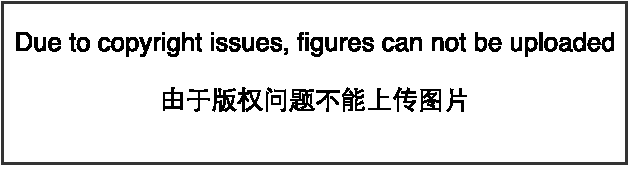
\includegraphics{figure.pdf}}
\else
\begin{tabular}{cc}
输入 & 重构 \\
\includegraphics[width=0.45\textwidth]{Chapter15/figures/ping_pong_input} &
\includegraphics[width=0.45\textwidth]{Chapter15/figures/ping_pong_reconstruction}
\end{tabular}
\fi
\caption{TODO}
\label{fig:chap15_pingpong}
\end{figure}

还有一些其他的突出性的定义。
例如,如果一组像素具有高度可识别的模式,那么即使该模式不涉及到极端的亮度或暗度,该模式还是会被认为非常突出。
实现这样一种定义突出的方法是使用最近开发的\firstgls{generative_adversarial_networks}\citep{Goodfellow-et-al-NIPS2014-small}。
在这种方法中,\gls{generative_model}被训练来愚弄\gls{feedforward_classifier}。
\gls{feedforward_classifier}尝试将来自生成模型的所有样本识别为假的,并将来自训练集合的所有样本识别为真的。
在这个框架中,\gls{feedforward_network}能够识别出的任何结构化模式都是非常突出的。
\gls{generative_adversarial_networks}会在第20.10.4节中更详细地介绍。
就现在的讨论而言,知道它能学习出什么是突出就可以了。
\cite{lotter2015unsupervised}表明,生成人类头部头像的模型在训练时使用\gls{mean_squared_error}往往会忽视耳朵,但是对抗式框架学习能够成功地生成耳朵。
因为耳朵与周围的皮肤相比不是非常明亮或黑暗,所以根据\gls{mean_squared_error}它们不是特别突出,但是它们高度可识别的形状和一致的位置意味着前向网络能够轻易地学习出如何检测它们,从而使得它们在生成式对抗框架下是高度突出的。
如\figref{fig:chap15_manface}所示。
\gls{generative_adversarial_networks}只是确定应该表示哪些因素的一小步。
我们期望未来的研究能够发现更好的方式来确定表示哪些因素,并且根据任务来发展表示不同因素的机制。

% -- 534 --

\begin{figure}[!htb]
\ifOpenSource
\centerline{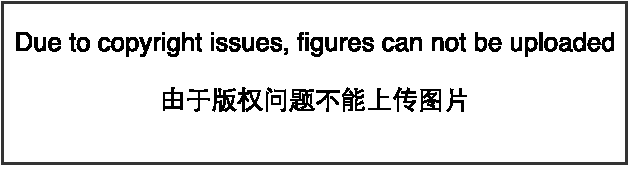
\includegraphics{figure.pdf}}
\else
\begin{tabular}{ccc}
真实图 & \glssymbol{mean_squared_error} & 对抗学习 \\
\includegraphics[width=0.3\textwidth]{Chapter15/figures/PGN_face1_GT} &
\includegraphics[width=0.3\textwidth]{Chapter15/figures/PGN_face1_MSE} &
\includegraphics[width=0.3\textwidth]{Chapter15/figures/PGN_face1_AL}
\end{tabular}
\fi
\caption{TODO}
\label{fig:chap15_manface}
\end{figure}

正如\cite{Janzing-et-al-ICML2012}指出,学习潜在因素的好处是,如果真实的生成过程中$\RVx$是结果,$\RVy$是原因,那么建模$p(\RVx \mid \RVy)$对于$p(\RVy)$的变化是鲁棒的。
如果因果关系被逆转,这是不对的,因为根据\gls{bayes_rule},$p(\RVx \mid \RVy)$将会对$p(\RVy)$的变化十分敏感。
很多时候,我们考虑不同领域(例如时间不稳定性或任务性质的变化)上分布的变化时,\emph{因果机制是保持不变的}(``宇宙定律不变''),而潜在因素的边缘分布是会变化的。
因此,通过学习试图恢复成因向量$\RVh$和$p(\RVx \mid \RVh)$的\gls{generative_model},可以期望最后的模型对所有种类的变化有更好的泛化和鲁棒性。

% -- 535 --

\section{\glsentrytext{distributed_representation}}
\label{sec:distributed_representation}
\gls{distributed_representation}的概念——由很多因素组合而成的表示,彼此可以分开设置——是\gls{representation_learning}最重要的工具之一。
\gls{distributed_representation}非常强大,因为他们能用具有$k$个值的$n$个特征去描述$k^n$个不同的概念。
正如我们在本书中看到的,具有多个\gls{hidden_unit}的\gls{NN}和具有多个\gls{latent_variable}的概率模型都利用了\gls{distributed_representation}的策略。
我们现在再介绍一个观察结果。
许多\gls{DL}算法基于的假设是,\gls{hidden_unit}能够学习出解释数据的潜在因果因素,见\secref{sec:semi_supervised_disentangling_of_causal_factors}中的讨论。
这种方法在\gls{distributed_representation}上是自然的,因为表示空间中的每个方向都对应着不同底层配置变量的值。

% -- 536 --

$n$维二元向量是一个\gls{distributed_representation}的示例,有$2^n$种配置,每一种都对应输入空间中的一个不同区域,如\figref{fig:chap15_distributed}所示。
这可以与\emph{符号表示}相比较,其中输入关联到单一符号或类别。
如果字典中有$n$个符号,那么可以想象有$n$个特征监测器,分别监测相关类别的存在。
在这种情况下,只有表示空间中$n$个不同配置才有可能在输入空间中刻画$n$个不同的区域,如\figref{fig:chap15_nondistributed}所示。
这样的符号表示也被称为\gls{one_hot}表示,因为它可以表示成各位排斥的$n$维二元向量(其中只有一位是激活的)。
符号表示是更广泛的非\gls{distributed_representation}中的一个具体示例,可以包含很多条目,但是每个条目没有显著意义的单独控制作用。

\begin{figure}[!htb]
\ifOpenSource
\centerline{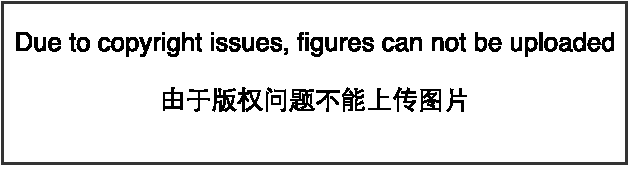
\includegraphics{figure.pdf}}
\else
\centerline{\includegraphics{Chapter15/figures/distributed}}
\fi
\caption{TODO}
\label{fig:chap15_distributed}
\end{figure}

\begin{figure}[!htb]
\ifOpenSource
\centerline{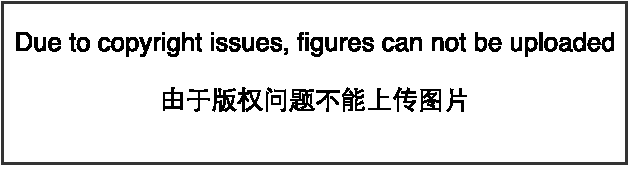
\includegraphics{figure.pdf}}
\else
\centerline{\includegraphics{Chapter15/figures/non_distributed}}
\fi
\caption{TODO}
\label{fig:chap15_nondistributed}
\end{figure}

以下是基于非\gls{distributed_representation}的学习算法的示例:
\begin{itemize}
	\item 聚类算法,包含$k$-均值算法:每个输入点恰好分配到一个类别。

	\item $k$-最近邻算法:给定一个输入,一个或几个模板或原型样本与之关联。
	在$k > 1$的情况下,多个值被用来描述每个输入,但是它们不能彼此分开控制,因此这不能算真正的\gls{distributed_representation}。

	\item 决策树:给定输入时,只有叶节点(和从根到叶节点的路径上的点)是被激活的。

	\item 高斯混合和专家混合:模板(聚类中心)或专家关联一个激活的\emph{程度}。
	和$k$-最近邻算法一样,每个输入用多个值表示,但是这些值不能轻易地彼此分开控制。

	\item 具有高斯核(或其他相似局部核)的\gls{kernel_machines}:尽管每个``\gls{support_vectors}''或模板样本的激活程度是连续值,但仍然会出现和高斯混合相同的问题。

	\item 基于\gls{n_gram}的语言或翻译模型:根据后缀的树结构划分上下文集合(符号序列)。
	例如,叶节点可能对应于最后两个单词$w_1$和$w_2$。
	树上的每个叶节点分别估计单独的参数(有些共享也是可能的)。
\end{itemize}

% -- 537 --

对于这些非分布式算法中的部分而言,有些输出并非是恒定的,而是在相邻区域之间内插。
参数(或样本)的数量和可定义区域的数量之间保持线性关系。


将\gls{distributed_representation}和符号表示区分开来的一个重要概念是,由不同概念之间的\emph{共享属性而产生的泛化}。
作为纯符号,``猫''和``狗''之间的距离和任意其他两种符号的距离一样。
然而,如果将它们与有意义的\gls{distributed_representation}相关联,那么关于猫的很多特点可以推广到狗,反之亦然。
例如,我们的\gls{distributed_representation}可能会包含诸如``是否具有皮毛''或``腿的数目''这类在``猫''和``狗''的嵌入上具有相同值的项。
正如\secref{sec:neural_language_models}所讨论的,作用于单词\gls{distributed_representation}的神经语言模型比其他直接对单词\gls{one_hot}表示进行操作的模型泛化得更好。
\gls{distributed_representation}具有丰富的\emph{相似性空间},语义上相近的概念(或输入)在距离上接近,这是纯粹的符号表示所缺少的特点。

% -- 539 --

何时使用\gls{distributed_representation}能够具有统计优势,以及为什么具有统计优势?
当一个明显复杂的结构可以用较少参数紧致地表示时,\gls{distributed_representation}具有统计上的优点。
一些传统的非分布式学习算法仅仅在平滑假设的情况下泛化能力比较好,也就是说如果$u\approx v$,那么学习到的目标函数$f$通常具有$f(u) \approx f(v)$的性质。
有许多方法来形式化这样一个假设,其结果是如果我们有一个样本$(x,y)$,并且我们知道$f(x) \approx y$,那么我们可以选取一个估计器$\hat{f}$近似地满足这些限制,并且当我们移动到附近的输入$x + \epsilon$,尽可能少地发生改变。
这个假设是非常有用的,但是它会承受\gls{curse_of_dimensionality}:
在很多不同区域上增加或减少很多次学习出一个目标函数\footnote{我们可能会想要学习一个能够区分指数级数量区域的函数:在$d$-维空间中,每维至少有两个不同的值。我们想要函数$f$区分这$2^d$个不同的区域,需要$O(2^d)$个训练样本},我们可能需要至少和可区分区域数量一样多的样本。
可以将每一个区域视为类别或符号:通过让每个符号(或区域)具有单独的自由度,我们可以学习出从符号映射到值的任意解码器。
然而,这不能推广到新区域的新符号上。


如果我们幸运的话,除了平滑之外,目标函数可能还有一些其他规律。
例如,具有\gls{max_pooling}的\gls{convolutional_network}
可以不考虑对象在图像中的位置(即使对象的空间变换不对应输入空间的平滑变换),而识别出对象。


让我们检查\gls{distributed_representation}学习算法的一个特殊情况,它通过对输入的线性函数进行阀值处理来提取二元特征。
该表示中的每个二元特征将$\SetR^d$分成一对半空间,如\figref{fig:chap15_distributed}所示。
$n$个半空间的指数级数量的交集确定了该\gls{distributed_representation}学习能够区分多少区域。
空间$\SetR^d$中的$n$个超平面的排列组合能够生成多少区间?
通过应用关于超平面交集的一般结果\citep{Zaslavsky-1975},我们可以展示\citep{Pascanu+et+al-ICLR2014b}这个二元特征表示能够区分的空间数量是
\begin{equation}
	\sum_{j=0}^d \binom{n}{j} = O(n^d)。
\end{equation}
因此,我们会发现输入大小呈指数级增长,\gls{hidden_unit}的数量呈多项式级增长。

% -- 540 --

这提供了一个几何说法来解释\gls{distributed_representation}的泛化能力:$O(nd)$个参数(空间$\SetR^d$中的$n$个线性阀值特征)能够明确表示输入空间中$O(n^d)$个区域。
如果我们没有对数据做任何假设,并且每个区域具有唯一的符号表示,每个符号使用单独的参数去识别$\SetR^d$中的对应区域,那么指定$O(n^d)$个区域需要$O(n^d)$个样本。
更一般地,我们对\gls{distributed_representation}中的每个特征使用非线性的可能连续的特征提取器,代替线性阀值单元,更加有利于体现\gls{distributed_representation}的优势。
在这种情况下,如果$k$个参数的参数变换可以学习输入空间中的$r$个区域($k\ll r$),如果学习这样的表示有助于感兴趣的任务,那么我们可以将这种方式潜在地推广到比非分布式设定更好的表示,我们只需要$O(r)$个样本来获得相同的特征,并将输入空间相关联地划分成$r$个区域。
使用较少的参数来表示模型意味着我们只需拟合较少的参数,因此只需要更少的训练样本去获得良好的泛化。


另一个解释基于\gls{distributed_representation}的模型泛化能力更好的说法是,尽管能够明确地编码这么多不同的区域,但它们的容量仍然是很有限的。
例如,线性阀值单位的\gls{NN}的\glssymbol{VC}维仅为$O(w\log w)$,其中$w$是权重的数目\citep{sontag1998vc}。
这种限制出现的原因是,虽然我们可以为表示空间分配非常多的唯一码,但是我们不能完全使用所有的码空间,也不能使用\gls{linear_classifier}学习出从表示空间$\Vh$到输出$\Vy$的任意函数映射。
因此使用与\gls{linear_classifier}相结合的\gls{distributed_representation}传达了一种先验信念,待识别的类在$\Vh$代表的潜在因素的函数下是线性可分的。
我们通常想要学习类别,例如所有绿色对象的所有图像集合,或是汽车的所有图像集合,但不会是需要非线性XOR逻辑的类别。
例如,我们通常不会将数据划分成所有红色汽车和绿色卡车作为一个集合,所有绿色汽车和红色卡车作为另一个集合。

% -- 541 --

到目前为止讨论的想法都是抽象的,但是它们可以通过实验验证。
\cite{Zhou-et-al-ICLR2015}发现,在ImageNet和Places基准数据集上训练的深度\gls{convolutional_network}中的\gls{hidden_unit}学习到的特征通常是可以解释的,对应人类自然分配的标签。
在实践中,\gls{hidden_unit}并不能总是学习出具有简单名称的事物,但有趣的是,这些会在计算机视觉深度网络的顶层附近出现。
这些特征的共同之处在于,我们可以想象\emph{学习其中的每个特征不需要知道所有其他特征的所有配置}。
\cite{radford2015unsupervised}展示生成模型可以学习人脸图像的表示,在表示空间中的不同方向捕获不同的潜在变化因素。
\figref{fig:chap15_generative_glasses}展示表示空间中的一个方向对应着该人是男性还是女性,而另一个方向对应着该人是否戴着眼镜。
这些特征都是自动发现的,而非先验固定的。
没有必要为\gls{hidden_unit}分类器提供标签:只要该任务需要这样的特征,\gls{GD}就能在感兴趣的目标函数上自然地学习出语义上有趣的特征。
我们可以学习出男性和女性之间的区别,或者是眼镜的存在与否,而不必通过涵盖所有这些值组合的样本来表征其他$n-1$个特征的所有配置。
这种形式的统计可分离性质能够泛化到训练期间从未见过的人。

\begin{figure}[!htb]
\ifOpenSource
\centerline{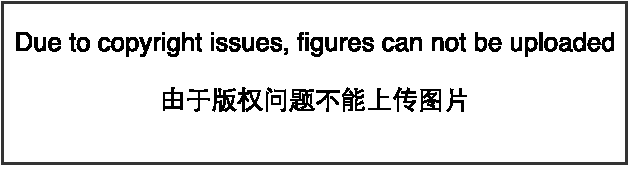
\includegraphics{figure.pdf}}
\else
\begin{tabular}{ccccccc}
\includegraphics[width=0.1\textwidth]{Chapter15/figures/man_with_glasses} &
- &
\includegraphics[width=0.1\textwidth]{Chapter15/figures/man_without_glasses} &
+ &
\includegraphics[width=0.1\textwidth]{Chapter15/figures/woman_without_glasses} &
= &
\includegraphics[width=0.3\textwidth]{Chapter15/figures/woman_with_glasses}
\end{tabular}
\fi
\caption{TODO}
\label{fig:chap15_generative_glasses}
\end{figure}
% -- 542 --


\section{得益于深度的指数增益}
\label{sec:exponential_gains_from_depth}
我们已经在\secref{sec:universal_approximation_properties_and_depth}中看到,\gls{MLP}是通用的近似器,一些函数能够用指数级小的\gls{deep_network}(相比于浅层网络)表示。
缩小模型规模能够提高统计效率。
在本节中,我们描述如何将类似结果更一般地应用于其他具有分布式隐藏表示的模型。


在\secref{sec:distributed_representation}中,我们看到了一个\gls{generative_model}的示例,能够学习人脸图像的解释性因素,包括性别以及是否佩戴眼镜。
完成这个任务的\gls{generative_model}基于一个\gls{DNN}。
浅层网络(例如线性网络)不能学习出这些抽象解释因素和图像像素之间的复杂关系。
在这个任务和其他\glssymbol{AI}任务中,彼此几乎独立,但仍然对应到有意义输入的因素,很有可能是高度抽象的,并且和输入呈高度非线性的关系。
我们认为这需要\emph{深度}\gls{distributed_representation},需要许多非线性组合来获得较高级的特征(被视为输入的函数)或因素(被视为生成原因)。


许多不同设置已经证明,
非线性和重用特征层次结构的组合来组织计算,可以使\gls{distributed_representation}获得指数级加速之外,还可以获得统计效率的指数级提升。
许多只有一个\gls{hidden_layer}的网络(例如,具有饱和非线性,布尔门,和/积,或\glssymbol{RBF}单元的网络)都可以被视为通用近似器。
在给定足够多\gls{hidden_unit}的情况下,通用近似器可以在任意非零允错级别近似一大类函数(包括所有连续函数)。
然而,\gls{hidden_unit}所需的数量可能会非常大。
关于深层架构的表达能力的理论结果表明,有些函数族可以有效地通过深度$k$层的网络架构表示,但是深度不够(深度为2或$k-1$)时会需要指数级(相对于输入大小而言)的\gls{hidden_unit}。

% -- 543 --

在\secref{sec:universal_approximation_properties_and_depth}中,我们看到确定性\gls{feedforward_network}是函数的\gls{universal_approximator}。
许多具有\gls{latent_variable}的单个\gls{hidden_layer}的\gls{structured_probabilistic_models}(包括\gls{RBM},\gls{DBN})是概率分布的\gls{universal_approximator}\citep{LeRoux-Bengio-2007-TR,Montufar-2011,Montufar-et-al-NIPS2014,Krause-et-al-ICML2013}。


在\secref{sec:universal_approximation_properties_and_depth}中,我们看到足够深的\gls{feedforward_network}会比深度不够的网络具有指数级优势。
这样的结果也能从诸如概率模型的其他模型中获得。
\firstgls{sum_product_network},或\glssymbol{sum_product_network}\citep{Poon+Domingos-2011}是这样的一种概率模型。
这些模型使用多项式电路来计算一组\gls{RV}的\gls{PD}。
\cite{Delalleau+Bengio-2011-small}表明存在一种\gls{PD},对\glssymbol{sum_product_network}的最小深度有要求,以避免模型规模呈指数级增长。
后来,\cite{Martens+Medabalimi-arxiv2014}表明,任意两个有限深度的\glssymbol{sum_product_network}之间都会存在显著差异,并且一些使\glssymbol{sum_product_network}易于处理的约束可能会限制其表示能力。


另一个有趣的进展是,一套和卷积网络相关的\gls{deep_circuit}族的表达能力的理论结果,即使让\gls{shadow_circuit}只去近似\gls{deep_circuit}计算的函数,也能突出反映\gls{deep_circuit}的指数级优势\citep{Cohen-et-al-arXiv2015}。
相比之下,以前的理论工作只研究了\gls{shadow_circuit}必须精确复制特定函数的情况。


\section{提供发现潜在原因的线索}
\label{sec:providing_clues_to_discover_underlying_causes}
我们回到最初的问题之一来结束本章:什么原因能够使一个表示比另一个表示更好?
首先在\secref{sec:semi_supervised_disentangling_of_causal_factors}中介绍的一个答案是,一个理想的表示能够区分生成数据的变化的潜在因果因素,特别是那些与我们的应用相关的因素。
\gls{representation_learning}的大多数策略都会引入一些有助于学习潜在变动因素的线索。
这些线索可以帮助\gls{learner}将这些观察到的因素与其他因素分开。
\gls{supervised_learning}提供了非常强的线索:每个观察向量$\Vx$的标签向量$\Vy$通常直接指定了至少一个变化因素。
更一般地,为了利用丰富的未标记数据,\gls{representation_learning}会使用关于潜在因素的其他不太直接的提示。
这些提示包含一些我们(学习算法的设计者)为了引导\gls{learner}而强加的隐式先验信念。
诸如\gls{no_free_lunch_theorem}的这些结果表明,正则化策略对于获得良好泛化是很有必要的。
当不可能找到一个普遍良好的\gls{regularization}策略时,\gls{DL}的一个目标是找到一套相当通用的\gls{regularization}策略,能够适用于各种各样的\glssymbol{AI}任务(类似于人和动物能够解决的任务)。

% -- 544 --

在此,我们提供了一些通用\gls{regularization}策略的列表。
该列表显然是不详尽的,但是给出了一些学习算法是如何发现潜在因素特征的具体示例。
该列表由\cite{Bengio-Courville-Vincent-TPAMI-2012}中\secref{sec:why_probability}提出,这里进行了部分拓展。
\begin{itemize}
	\item \emph{平滑}:假设对于单位$\Vd$和小量$\epsilon$有$f(\Vx + \epsilon \Vd) \approx f(\Vx)$。
	这个假设允许\gls{learner}从训练样本泛化到输入空间中附近的点。
	许多\gls{ML}算法都利用了这个想法,但它不能克服\gls{curse_of_dimensionality}难题。


	\item \emph{线性}:很多学习算法假定一些变量之间的关系是线性的。
	这使得算法能够预测远离观测数据的点,但有时可能会导致一些极端的预测。
	大多数简单的学习算法不会做平滑假设,而会做线性假设。
	这些假设实际上是不同的——具有很大权重的线性函数在高维空间中可能不是非常平滑的。
	参看\cite{Goodfellow-2015-adversarial}了解关于线性假设局限性的进一步讨论。


	\item \emph{多个解释因素}:许多\gls{representation_learning}算法受激励于这样的假设,数据是由多个潜在解释性因素生成的,并且给定每一个因素的状态,大多数任务都能轻易解决。
	\secref{sec:semi_supervised_disentangling_of_causal_factors}描述了这种观点如何通过\gls{representation_learning}促进\gls{semi_supervised_learning}的。
	学习$p(\Vx)$的结构要求学习出一些对建模$p(\Vy\mid\Vx)$同样有用的特征,因为它们都涉及到相同的潜在解释因素。
	\secref{sec:distributed_representation}介绍了这种观点如何激发\gls{distributed_representation}的使用,表示空间中不同的方向对应着不同的变化因素。


	\item \emph{因果因素}:该模型认为学习到的表示所描述的变量是观察数据$\Vx$的成因,而并非反过来。
	正如\secref{sec:semi_supervised_disentangling_of_causal_factors}中讨论的,这对于\gls{semi_supervised_learning}是有利的,当潜在成因上的分布发生改变,或者我们应用模型到一个新的任务上时,学习到的模型都会更加鲁棒。

% -- 545 --

	\item \emph{深度,或者解释因素的层次组织}:层次结构的简单概念能够定义高级抽象概念。
	从另一个角度来看,深层架构表达了我们认为任务应该由多个程序步骤完成的观念,每一个步骤回溯到先前步骤完成处理的输出。


	\item \emph{任务间共享因素}:
	当多个对应到不同变量$\RSy_i$的任务共享相同的输入$\RVx$时,或者当每个任务关联到全局输入$\RVx$的子集或者函数$f^{(i)}(\RVx)$时,我们会假设每个变量$\RSy_i$关联到来自相关因素$\RVh$公共池的不同子集。
	因为这些子集有重叠,所以通过共享的中间表示$ P(\RVh \mid \RVx)$来学习所有的$P(\RSy_i \mid \RVx)$能够使任务间共享统计信息。


	\item \emph{\gls{manifold}}:概率质量集中,并且集中区域是局部连通的,且占据很小的体积。
	在连续情况下,这些区域可以用比数据所在原始空间低很多维的低维\gls{manifold}来近似。
	很多\gls{ML}算法只在这些\gls{manifold}上有效\citep{Goodfellow-2015-adversarial}。
	一些\gls{ML}算法,特别是\gls{AE},会试图学习\gls{manifold}的结构。


	\item \emph{自然聚类}:很多\gls{ML}算法假设输入空间中的每个连通\gls{manifold}都是一个单独的类。
	数据分布在许多个不连通的\gls{manifold}上,但相同\gls{manifold}上数据的类别是相同的。
	这个假设激励了各种学习算法,包括\gls{tangent_propagation},\gls{double_backprop},\gls{manifold_tangent_classifier}和\gls{adversarial_training}。


	\item \emph{时间和空间相干性}:慢特征分析和相关的算法假设,最重要的解释因素随时间变化很缓慢,或者至少假设预测真实的解释因素比预测诸如像素值这类原始观察会更容易些。
	参考\secref{sec:slow_feature_analysis},进一步了解这个方法。


	\item \emph{稀疏性}:假设大部分特征和大部分输入不相关——在表示猫的图像时,没有必要使用大象的特征。
	因此,我们可以强加一个先验,任何可以解释为``存在''或``不存在''的特征在大多数样本中都是不需要的。

% -- 546 --

	\item \emph{简化因素依赖性}:在良好的高级表示中,因素会通过简单的依赖相互关联。
	边缘独立可能是最简单的,$P(\RVh) = \prod_i P(\RVh_i)$。线性依赖或浅层\gls{AE}也是合理的假设。
	这可以在许多物理定律中看出来,在学习到的表示上使用线性预测器或分解先验。
\end{itemize}


\gls{representation_learning}的概念将所有的\gls{DL}形式联系到了一起。
\gls{feedforward_network}和\gls{recurrent_network},\gls{AE}和深度概率模型都在学习和使用表示。
学习最佳表示仍然是一个令人兴奋的研究方向。

% -- 547 --
